\documentclass[10pt,a4paper]{article}
\usepackage[utf8]{inputenc}
\usepackage[T1]{fontenc}
\usepackage{amsmath}
\usepackage{amsfonts}
\usepackage{amssymb}
\usepackage{graphicx}
\usepackage{listings}
\usepackage{float}
\usepackage{multirow}
\usepackage{subcaption}
\usepackage[table]{xcolor}
\usepackage[labelformat=parens,labelsep=quad,skip=3pt]{caption}


\begin{document}
	\title{Homework 3 - Frame Based Scheduling}
	\makeatletter
	
	\author{Zackary McClamma\thanks{University of Dayton}
		\thanks{Dept. of Electrical and Computer
			Engineering, University of Dayton, 300 College Park, Dayton, OH
			45469-0226, U.S.A. E-mail:
			mcclammaz1@udayton.edu}}
	
	\makeatother
	
	\date{\today}
	
	\maketitle
	\section{Introduction}
	In this homework assignment consisted of adding all of the available 7-segment displays (8 total), a switch for each display, and a timer. It also included creating software that uses a timer interrupt to trigger an ISR. The ISR uses a frame based schedule to poll the state of the switches and determine if the value on the 7-segment display will be incremented or decremented. This assignment also required the calculation of the load for each individual task and the total load on the processor.
	
	\section{System Design}
 	This system uses a total of 16 peripherals, one clock, and of course the Nios II processor. There are a total of 8 seven segment displays and 8 switches. Each seven segment display is 'assigned' a switch and the state of the switch will determine what the display should output. Every 250ms a timer interrupt is triggered and the ISR executes a frame, the ISR cycles through and increments the frame count every time the interrupt is triggered, when the last frame is triggered the ISR resets the frame count and starts from the first frame (in this scenario there are 4 frames total). The switches have two possible states (on/off i.e. 1 or 0), every interrupt a set of the switches is polled and if the stat of the switch is 1 then the seven segment display is incremented, if it is zero then the display is decremented.

	
	\section{Theory of Operation}
	Below is the block diagram for this assignment it is fairly similar to the previous two assignments with the main difference being in this case that the interrupt is synchronous and is based of of the timer. As can be seen from \ref{block} the timer triggers an interrupt which causes the processor to check the state of the switches (which switches are polled depends on which frame is being executed). Dependent on the state of the switch the corresponding display will be incremented (switch state is 1) or decremented (switch state is 0).
	\begin{figure}[H]
		\centering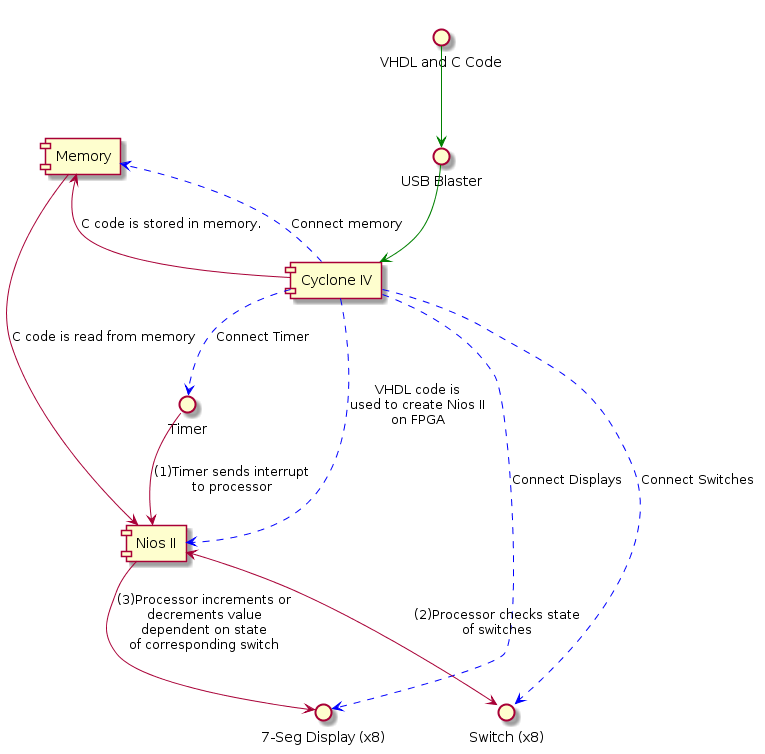
\includegraphics[width=15cm]{HW3_Block.png}
		\caption{Embedded System Block Diagram}
		\label{block}
	\end{figure}
	\subsection{Tables}
	Below are a couple of tables outlining the structure of the frames in this project, \ref{taskDes} is the breakdown of each individual frame and \ref{frameSch} is the frame schedule. As you can see from \ref{taskDes} the system load for this program is below 2\% this is to be expected as this is a simple program that only consists of a timer interrupt that triggers the reading of a memory address and an increment or decrement of another address.
	\begin{center}
		\begin{table}[ht]
			\centering
			\caption{Task Information}
			\begin{tabular}{l*{5}{c}r}
				\hline
				Task Number & Rate (Hz) & Duration(ms) & Period(ms) & Load \\
				\hline
				0  & 4 & 1 & 250 & .004  \\
				1 & 4 & 1 & 250 &  .004  \\
				2  & 2 & 1 & 500 & .002 \\
				3  & 2 & 1 & 500 & .002   \\
				4  & 2 & .5 & 500 & .002   \\
				5  & 2 & .5 & 500 & .002   \\
				6  & 1 & .5 & 1000 & .001   \\
				7  & 1 & .5 & 1000 &  .001  \\
				\hline
				System Load & & & & 1.8\%
				\label{taskDes}
			\end{tabular}
		\end{table}
	
	\begin{table}[h]
		\centering
		\caption{Frame Schedule}
		\begin{tabular}{l*{5}{c}r}
			\hline
			\multicolumn{5}{c}{Frames} \\
			\hline
			& 1 & 2 & 3 & 4 \\
			\hline
			\multirow{5}{*}{Tasks} \\
			& 0 & 0 & 0 & 0 \\
			& 1 & 1 & 1 & 1 \\
			& 2 & 4 & 2 & 4 \\
			& 3 & 5 & 3 & 5 \\
			& 6 & 7 &   &   \\
			\hline
			\label{frameSch}
		\end{tabular}
	\end{table}
	\end{center}

	\section{Results}
	The results of this project are difficult to capture in writing or with images, so I have included a video of the functioning project with the submission of this document. The end result functioned as I expected (as outlined in the assignment description).

	\section{Conclusion}
	This assignment was beneficial in understanding how to use timer interrupts with the Nios II processor. This was also the first assignment where I worked with vectored peripherals and I think that it made my code much more condensed and easier to work with. The only issues I have with my final product is the way that I execute the ISR, I was trying to find a way to return to main and run the frames but I had issues with the ISR triggering again before the code could execute. I attempted to disable the ISR in the meantime but to no avail. To circumvent this i put the frame execution code in the ISR and those frames call external functions to check the switches and change the displays. My goal was to use less code in the ISR because I know that when schedules get more complex having too much code in an ISR can cause issues, but in this case executing code in the ISR shouldn't cause any issues, as this is a simple program and is not doing any complex operations.
	\clearpage
	\appendix
	\section{\\VHDL Code}
	\lstinputlisting[language=VHDL]{homework3.vhd}
	
	\section{\\C Code}
	\subsection{Headers}
	\lstinputlisting[language=C]{hw3.h}
	
	\subsection{Source}
	\lstinputlisting[language=C]{main.c}
\end{document}